\documentclass[11pt,fleqn]{article}

\setlength {\topmargin} {-.15in}
\setlength {\textheight} {8.6in}

\usepackage{amsmath}
\usepackage{amssymb}
\usepackage{amsthm}
\usepackage{url}
\usepackage{color}
\usepackage{tikz}
\usetikzlibrary{automata,positioning,arrows}

\setlength {\topmargin} {-.15in}
\setlength {\textheight} {8.6in}

\renewcommand{\labelenumi}{\theenumi.}
\renewcommand{\labelenumii}{\theenumii.}
\renewcommand{\labelenumiii}{\theenumiii.}
\newcommand{\be}{\begin{enumerate}}
	\newcommand{\ee}{\end{enumerate}}
\newcommand{\bi}{\begin{itemize}}
	\newcommand{\ei}{\end{itemize}}
\newcommand{\bc}{\begin{center}}
	\newcommand{\ec}{\end{center}}
\newcommand{\bsp}{\begin{sloppypar}}
	\newcommand{\esp}{\end{sloppypar}}
\newcommand{\mname}[1]{\mbox{\sf #1}}
\newcommand{\sB}{\mbox{$\cal B$}}
\newcommand{\sC}{\mbox{$\cal C$}}
\newcommand{\sF}{\mbox{$\cal F$}}
\newcommand{\sM}{\mbox{$\cal M$}}
\newcommand{\sP}{\mbox{$\cal P$}}
\newcommand{\sV}{\mbox{$\cal V$}}
\newcommand{\set}[1]{{\{ #1 \}}}
\newcommand{\Neg}{\neg}
\ifdefined \And
\renewcommand{\And}{\wedge}
\else
\newcommand{\And}{\wedge}
\fi
\newcommand{\Or}{\vee}
\newcommand{\Implies}{\Rightarrow}
\newcommand{\Iff}{\LeftRightarrow}
\newcommand{\Forall}{\forall}
\newcommand{\ForallApp}{\forall\,}
\newcommand{\Forsome}{\exists}
\newcommand{\ForsomeApp}{\exists\,}
\newcommand{\mdot}{\mathrel.}
\newcommand{\eps}{\epsilon}
\newcommand{\pnote}[1]{\langle \mbox{#1} \rangle}


\begin{document}

\begin{center}

{\large \textbf{COMPSCI/SFWRENG 2FA3}}\\[2mm]
{\large \textbf{Discrete Mathematics with Applications II}}\\[2mm]
{\large \textbf{Winter 2021}}\\[8mm]
{\huge \textbf{Assignment 4}}\\[6mm]
{\large \textbf{Dr.~William M. Farmer and Dr.~Mehrnoosh Askarpour}}\\[2mm]
{\large \textbf{McMaster University}}\\[6mm]
{\large Revised: February 23, 2021}

\end{center}

\medskip

Assignment 4 consists of two problems.  You must write your solutions
to the problems using LaTeX.

Please submit Assignment~4 as two files,
\texttt{Assignment\_4\_\emph{YourMacID}.tex} and
\texttt{Assignment\_4\_\emph{YourMacID}.pdf}, to the Assignment~4
folder on Avenue under Assessments/Assignments.
\texttt{\emph{YourMacID}} must be your personal MacID (written without
capitalization).  The \texttt{Assignment\_4\_\emph{YourMacID}.tex}
file is a copy of the LaTeX source file for this assignment
(\texttt{Assignment\_4.tex} found on Avenue under
Contents/Assignments) with your solution entered after each problem.
The \texttt{Assignment\_4\_\emph{YourMacID}.pdf} is the PDF output
produced by executing

\begin{itemize}

  \item[] \texttt{pdflatex Assignment\_4\_\emph{YourMacID}}

\end{itemize}

This assignment is due \textbf{Sunday, February 28, 2021 before
  midnight.}  You are allow to submit the assignment multiple times,
but only the last submission will be marked.  \textbf{Late submissions
  and files that are not named exactly as specified above will not be
  accepted!}  It is suggested that you submit your preliminary
\texttt{Assignment\_4\_\emph{YourMacID}.tex} and
\texttt{Assignment\_4\_\emph{YourMacID}.pdf} files well before the
deadline so that your mark is not zero if, e.g., your computer fails
at 11:50 PM on February 28.

\textbf{Although you are allowed to receive help from the
  instructional staff and other students, your submission must be your
  own work.  Copying will be treated as academic dishonesty! If any of
  the ideas used in your submission were obtained from other students
  or sources outside of the lectures and tutorials, you must
  acknowledge where or from whom these ideas were obtained.}

\newpage

\subsection*{Presenting DFAs and NFAs Transition Diagrams}

In this assignment you are asked to present DFAs as transition
diagrams.  You are can do this in one of two ways.

The first way is to present the diagram using the LaTeX graphics
package TikZ.  The TikZ code can either be written by hand or
automatically generated using the finsm system available at
\texttt{http:finsm.io}.

Here are some examples of how it can be used to create
DFA and NFA transition diagrams that appear in the lectures slides:

\begin{center}
\begin{tikzpicture}[shorten >=1pt,node distance=2.5cm,on grid,auto] 
   \node[state, initial, thick] (q_0)   {$q_0$}; 
   \node[state, thick] (q_1) [right=of q_0] {$q_1$}; 
   \node[state, thick] (q_2) [right=of q_1] {$q_2$}; 
   \node[state, accepting, thick] (q_3) [right=of q_2] {$q_3$};
    \path[->, thick, >=stealth] 
    (q_0) edge [bend left, above] node {$a$} (q_1)
          edge [loop, above] node {$b$} (q_2)
    (q_1) edge [bend left, above] node {$a$} (q_2)
          edge [bend left, above] node {$b$} (q_0)
    (q_2) edge [bend left, above] node {$a$} (q_3) 
          edge [bend left, below]  node {$b$} (q_0)
    (q_3) edge [loop, above] node {$a,b$} (q_2); 
\end{tikzpicture}
\end{center}

\begin{center}
\begin{tikzpicture}[shorten >=1pt,node distance=4cm,on grid,auto] 
   \node[state, initial, accepting, thick] (q_0)   {$q_0$}; 
   \node[state, thick] (q_1) [right=of q_0] {$q_1$}; 
   \node[state, thick] (q_2) [below=of q_0] {$q_2$}; 
   \node[state, thick] (q_3) [right=of q_2] {$q_3$};
    \path[->, thick, >=stealth] 
    (q_0) edge [bend left, above] node {1} (q_1)
          edge [bend left, right] node {0} (q_2)
    (q_1) edge [bend left, below] node {1} (q_0)
          edge [bend left, right] node {0} (q_3)
    (q_2) edge [bend left, above] node {1} (q_3) 
          edge [bend left, left]  node {0} (q_0)
    (q_3) edge [bend left, below] node {1} (q_2) 
          edge [bend left, left]  node {0} (q_1);
\end{tikzpicture}
\end{center}

\begin{center}
\begin{tikzpicture}[shorten >=1pt,node distance=1.7cm,on grid,auto] 
   \node[state, initial, thick] (q_0)   {$q_0$}; 
   \node[state, thick] (q_1) [right=of q_0] {$q_1$}; 
   \node[state, thick] (q_2) [right=of q_1] {$q_2$}; 
   \node[state, thick] (q_3) [right=of q_2] {$q_3$};
   \node[state, thick] (q_4) [right=of q_3] {$q_4$};
   \node[state, thick, accepting] (q_5) [right=of q_4] {$q_5$};
    \path[->, thick, >=stealth] 
    (q_0) edge [loop, above] node {0,1} (q_1)
          edge [right, above] node {1} (q_1)
    (q_1) edge [right, above] node {0,1} (q_2)
    (q_2) edge [right, above] node {0,1} (q_3)
    (q_3) edge [right, above] node {0,1} (q_4)
    (q_4) edge [right, above] node {0,1} (q_5);
\end{tikzpicture}
\end{center}

The second way is to take a picture of a hand-written transition
diagram and then embed it into your assignment using the following
LaTeX code:
\begin{verbatim}
\begin{center}
\includegraphics[scale = 0.5]{diagram.jpg}
\end{center}
\end{verbatim}
Please make sure your diagram is legible.

\subsection*{Problems}

\be

  \item \textbf{[10 points]} Construct a deterministic finite
    automaton (DFA) $A$ for the alphabet $\Sigma = \set{0,1}$ such
    that $L(A)$ is the set of all strings $x$ in $\Sigma^*$ for which
    $\#0(x)$ is even and $\#1(x)$ is divisible by 3.  Present $A$ as a
    transition diagram.

  \textcolor{blue}{\textbf{Qiang Gao, gaoq20, and 2/28/2021}}\\
  \begin{verbatim}
  \begin{center}
  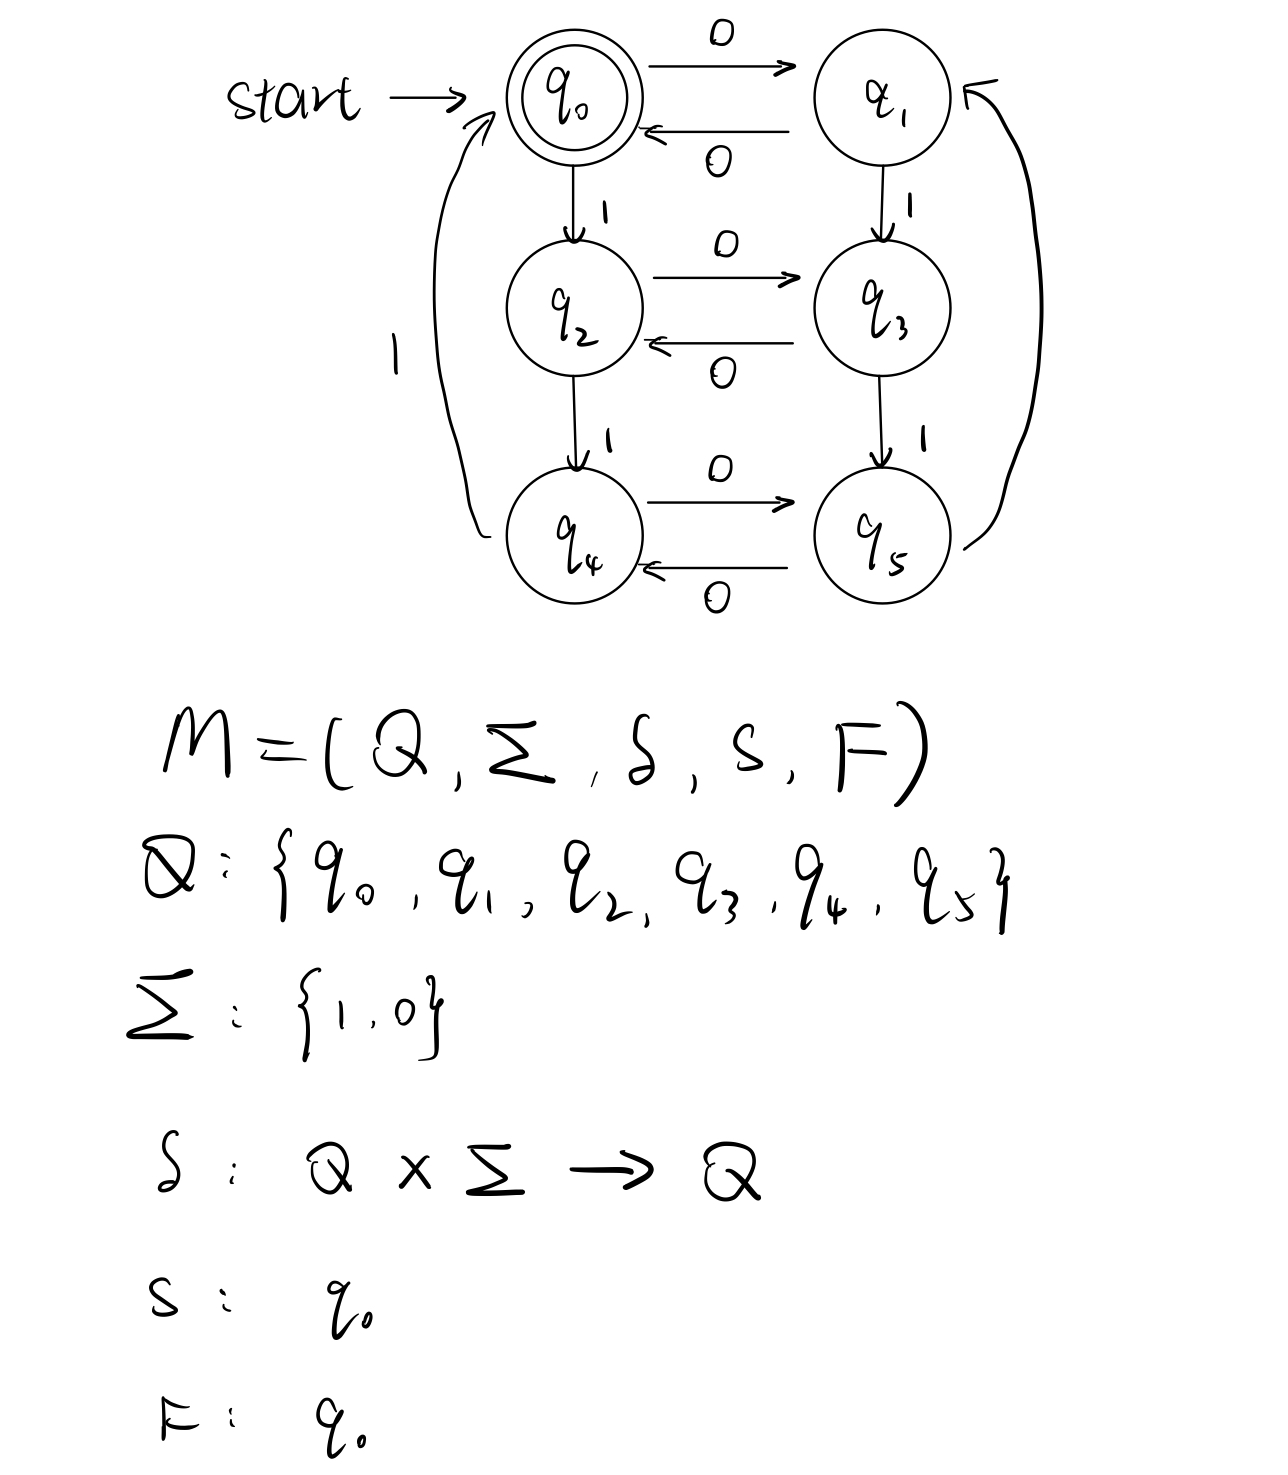
\includegraphics[scale = 0.5]{微信图片_20210301104229.jpg}
  \end{center}
  \end{verbatim}


  \item \textbf{[10 points]} Let $B$ be the DFA given by the following
    transition diagram:
	\begin{center}
	\begin{tikzpicture}[]
		\node[thick,initial,state] (q0) {$q_{0}$};
		\node[thick,accepting, state] (q1)  [right= of q0]{$q_{1}$};
		\node[thick,state] (q2)  [right= of q1]{$q_{2}$};
		\path[->, thick, >=stealth]
		(q0) edge [bend left,above] node {$1$} (q1)
		edge [loop above]   node         {0} ()
		(q1) edge [bend left,above] node {$0$} (q0)
		edge [bend left,above] node {$1$} (q2)
		(q2) edge [bend left,above] node {$1$} (q1)
		edge [bend left = 40, below] node {$0$} (q0)
		;
	\end{tikzpicture}
        \end{center}

   Prove that $L(B)$ is the language of all binary strings that end
   with an odd number of $1$s.  Hint: Use weak induction on the length
   of the input string, and let $P(n)$ be the statement that, for all
   input strings $w$ with $|w| = n$, the following conditions hold:

   \be

     \item If $\delta^*(q_0,w) = q_0$, then $w$ is $\epsilon$ or ends
       with $0$.

     \item If $\delta^*(q_0,w) = q_1$, then $w$ ends with an odd
       number of $1$s.

     \item If $\delta^*(q_0,w) = q_2$, then $w$ ends
       with an even number of $1$s.

   \ee
	
   \textcolor{blue}{\textbf{Qiang Gao, gaoq20, and 2/28/2021}}\\
   \begin{proof}
    \\\\
    We will prove $P(n)$ by weak induction.
    \\\\
    \medskip
    \emph{Base case}: 
    \\\\
    \emph{case 1}: $n = 0, w = \epsilon$
    \\\\
    From the graph, we can see that $\delta^*(q_0,\epsilon) = q_0$. Also, $w = \epsilon$. Therefore, a holds.
    \\\\
    \emph{case 2a}: $n = 1, w = 0$
    \\\\
    From the graph, we can see that $\delta^*(q_0,0) = q_0$. Also, 0 ends with 0. Therefore, a holds.
    \\\\
    \emph{case 2b}: $n = 1, w = 1$
    \\\\
    From the graph, we can see that $\delta^*(q_0,1) = q_1$. Also, 1 ends with an odd number of 1s. Therefore, b holds.
    \\\\
    \emph{case 3a}: $n = 2, w = 00$
    \\\\
    From the graph, we can see that $\delta^*(q_0,00) = q_0$. Also, 00 ends with 0. Therefore, a holds.
    \\\\
    \emph{case 3b}: $n = 2, w = 01$
    \\\\
    From the graph, we can see that $\delta^*(q_0,01) = q_1$. Also, 01 ends with an odd number of 1s. Therefore, b holds.
    \\\\
    \emph{case 3c}: $n = 2, w = 10$
    \\\\
    From the graph, we can see that $\delta^*(q_0,10) = q_0$. Also, 10 ends with 0. Therefore, a holds.
    \\\\
    \emph{case 3d}: $n = 2, w = 11$
    \\\\
    From the graph, we can see that $\delta^*(q_0,11) = q_2$. Also, 11 ends with an even number of 1s. Therefore, c holds.
    \medskip
    \\\\
    \\\\
    \emph{Induction step}: We show $P(n + 1)$ assuming $P(n)$.
    \\\\
    \emph{case 1a}: $\delta^*(q_0,w) = q_0$, prove $w0$
    \\\\
    By the definition of $\delta^*$, $\delta^*(q_0,w0)$ = $\delta(\delta^*(q_0,w),0)$. By assumption, $\delta(\delta^*(q_0,w),0)$ = $\delta(q_0,0)$. 
    From the graph,$\delta(q_0,0)$ = $q_0$. So, $\delta^*(q_0,w0)$ = $q_0$.
    By induction hypothesis, $w$ ends with 0, so $w0$ also ends with 0. Therefore, a holds.
    \\\\
    \emph{case 1b}: $\delta^*(q_0,w) = q_0$, prove $w1$
    \\\\
    By the definition of $\delta^*$, $\delta^*(q_0,w1)$ = $\delta(\delta^*(q_0,w),1)$. By assumption, $\delta(\delta^*(q_0,w),1)$ = $\delta(q_0,1)$. 
    From the graph,$\delta(q_0,1)$ = $q_1$. So, $\delta^*(q_0,w1)$ = $q_1$.
    By induction hypothesis, $w$ ends with 0, so $w1$ ends with 1(an odd number of 1s). Therefore, b holds.
    \\\\
    \emph{case 2a}: $\delta^*(q_0,w) = q_1$, prove $w0$
    \\\\
    By the definition of $\delta^*$, $\delta^*(q_0,w0)$ = $\delta(\delta^*(q_0,w),0)$. By assumption, $\delta(\delta^*(q_0,w),0)$ = $\delta(q_1,0)$. 
    From the graph,$\delta(q_1,0)$ = $q_0$. So, $\delta^*(q_0,w0)$ = $q_0$.
    By induction hypothesis, $w$ ends with an odd number of 1s, so $w0$ ends with 0. Therefore, a holds.
    \\\\
    \emph{case 2b}: $\delta^*(q_0,w) = q_1$, prove $w1$
    \\\\
    By the definition of $\delta^*$, $\delta^*(q_0,w1)$ = $\delta(\delta^*(q_0,w),1)$. By assumption, $\delta(\delta^*(q_0,w),1)$ = $\delta(q_1,1)$. 
    From the graph,$\delta(q_1,1)$ = $q_2$. So, $\delta^*(q_0,w1)$ = $q_2$.
    By induction hypothesis, $w$ ends with an odd number of 1s, so $w1$ ends with an even number of 1s since an odd number plus 1 is an even number. Therefore, c holds.
    \\\\
    \emph{case 3a}: $\delta^*(q_0,w) = q_2$, prove $w0$
    \\\\
    By the definition of $\delta^*$, $\delta^*(q_0,w0)$ = $\delta(\delta^*(q_0,w),0)$. By assumption, $\delta(\delta^*(q_0,w),0)$ = $\delta(q_2,0)$. 
    From the graph,$\delta(q_2,0)$ = $q_0$. So, $\delta^*(q_0,w0)$ = $q_0$.
    By induction hypothesis, $w$ ends with an even number of 1s, so $w0$ ends with 0. Therefore, a holds.
    \\\\
    \emph{case 3b}: $\delta^*(q_0,w) = q_2$, prove $w1$
    \\\\
    By the definition of $\delta^*$, $\delta^*(q_0,w1)$ = $\delta(\delta^*(q_0,w),1)$. By assumption, $\delta(\delta^*(q_0,w),1)$ = $\delta(q_2,1)$. 
    From the graph,$\delta(q_2,1)$ = $q_1$. So, $\delta^*(q_0,w1)$ = $q_1$.
    By induction hypothesis, $w$ ends with an even number of 1s, so $w1$ ends with an odd number of 1s since an even number plus 1 is an odd number. Therefore, b holds.
    \\\\
    $P(n + 1)$ holds.
    \medskip
    
    Therefore, $L(B)$ is the language of all binary strings that end
    with an odd number of $1$s.
    \end{proof}
      \bigskip

\ee

\end{document}


